\documentclass{article}
\usepackage{amsmath}
\usepackage{tikz}
\usetikzlibrary{arrows.meta}

\begin{document}

\begin{figure}[h]
    \centering
    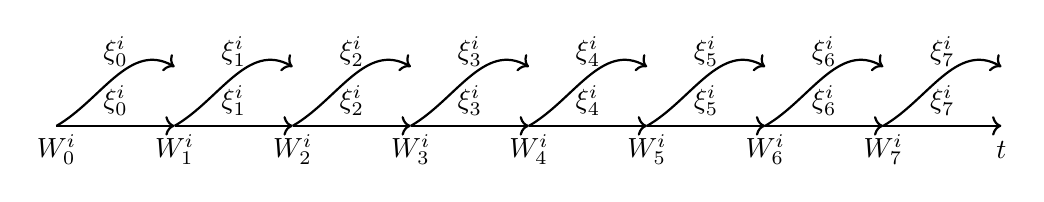
\begin{tikzpicture}[scale=1.5]
        % Nodes representing W_t^i values
        \foreach \i in {0,...,7} {
            \node at (\i,-0.2) {$W_\i^i$};
        }
        \node at (8,-0.2) {$t$};

        % Edges with Gaussian variables
        \draw[->, thick] (0,0) -- node[above] {$\xi_0^i$} (1,0);
        \draw[->, thick] (1,0) -- node[above] {$\xi_1^i$} (2,0);
        \draw[->, thick] (2,0) -- node[above] {$\xi_2^i$} (3,0);
        \draw[->, thick] (3,0) -- node[above] {$\xi_3^i$} (4,0);
        \draw[->, thick] (4,0) -- node[above] {$\xi_4^i$} (5,0);
        \draw[->, thick] (5,0) -- node[above] {$\xi_5^i$} (6,0);
        \draw[->, thick] (6,0) -- node[above] {$\xi_6^i$} (7,0);
        \draw[->, thick] (7,0) -- node[above] {$\xi_7^i$} (8,0);

        % Arrows indicating the path
        \draw[->, thick] (0,0) to[out=30,in=150] node[above] {$\xi_0^i$} (1,0.5);
        \draw[->, thick] (1,0) to[out=30,in=150] node[above] {$\xi_1^i$} (2,0.5);
        \draw[->, thick] (2,0) to[out=30,in=150] node[above] {$\xi_2^i$} (3,0.5);
        \draw[->, thick] (3,0) to[out=30,in=150] node[above] {$\xi_3^i$} (4,0.5);
        \draw[->, thick] (4,0) to[out=30,in=150] node[above] {$\xi_4^i$} (5,0.5);
        \draw[->, thick] (5,0) to[out=30,in=150] node[above] {$\xi_5^i$} (6,0.5);
        \draw[->, thick] (6,0) to[out=30,in=150] node[above] {$\xi_6^i$} (7,0.5);
        \draw[->, thick] (7,0) to[out=30,in=150] node[above] {$\xi_7^i$} (8,0.5);
    \end{tikzpicture}
    \caption{An illustration of the definition of $W_t^i$ for $i\in [K]$. The value of $W_t^i$ is obtained by summing the i.i.d. Gaussian variables $\xi_{t'}^i$'s on the edges along the path from $W_0^i$, i.e. summing over all $t'\in \mc S(t) \cup \{t\} \setminus \{0\}$. For example, $W_7^i=\xi_4^i +\xi_6^i+\xi_7^i$.}
    \label{fig:w_t_i}
\end{figure}

\end{document}